
\begin{frame}{Système de mesure externe}
    \begin{columns}
        \begin{column}{0.5\linewidth}
            \begin{block}{Capture de mouvements (\textit{mocap})}
                Mesure externe de la pose absolue 
            \end{block}
            \begin{itemize}
                \item Haute fréquence ($100$~Hz)
                \item Bonne précision (millimètre)
            \end{itemize}
            Mais :
            \begin{itemize}
                \item Matériel \og encombrant \fg
            \end{itemize}
            \vspace{1em}
            $\Longrightarrow$ Mesure déplacements égocentriques
        \end{column}
        \begin{column}{0.5\linewidth}
            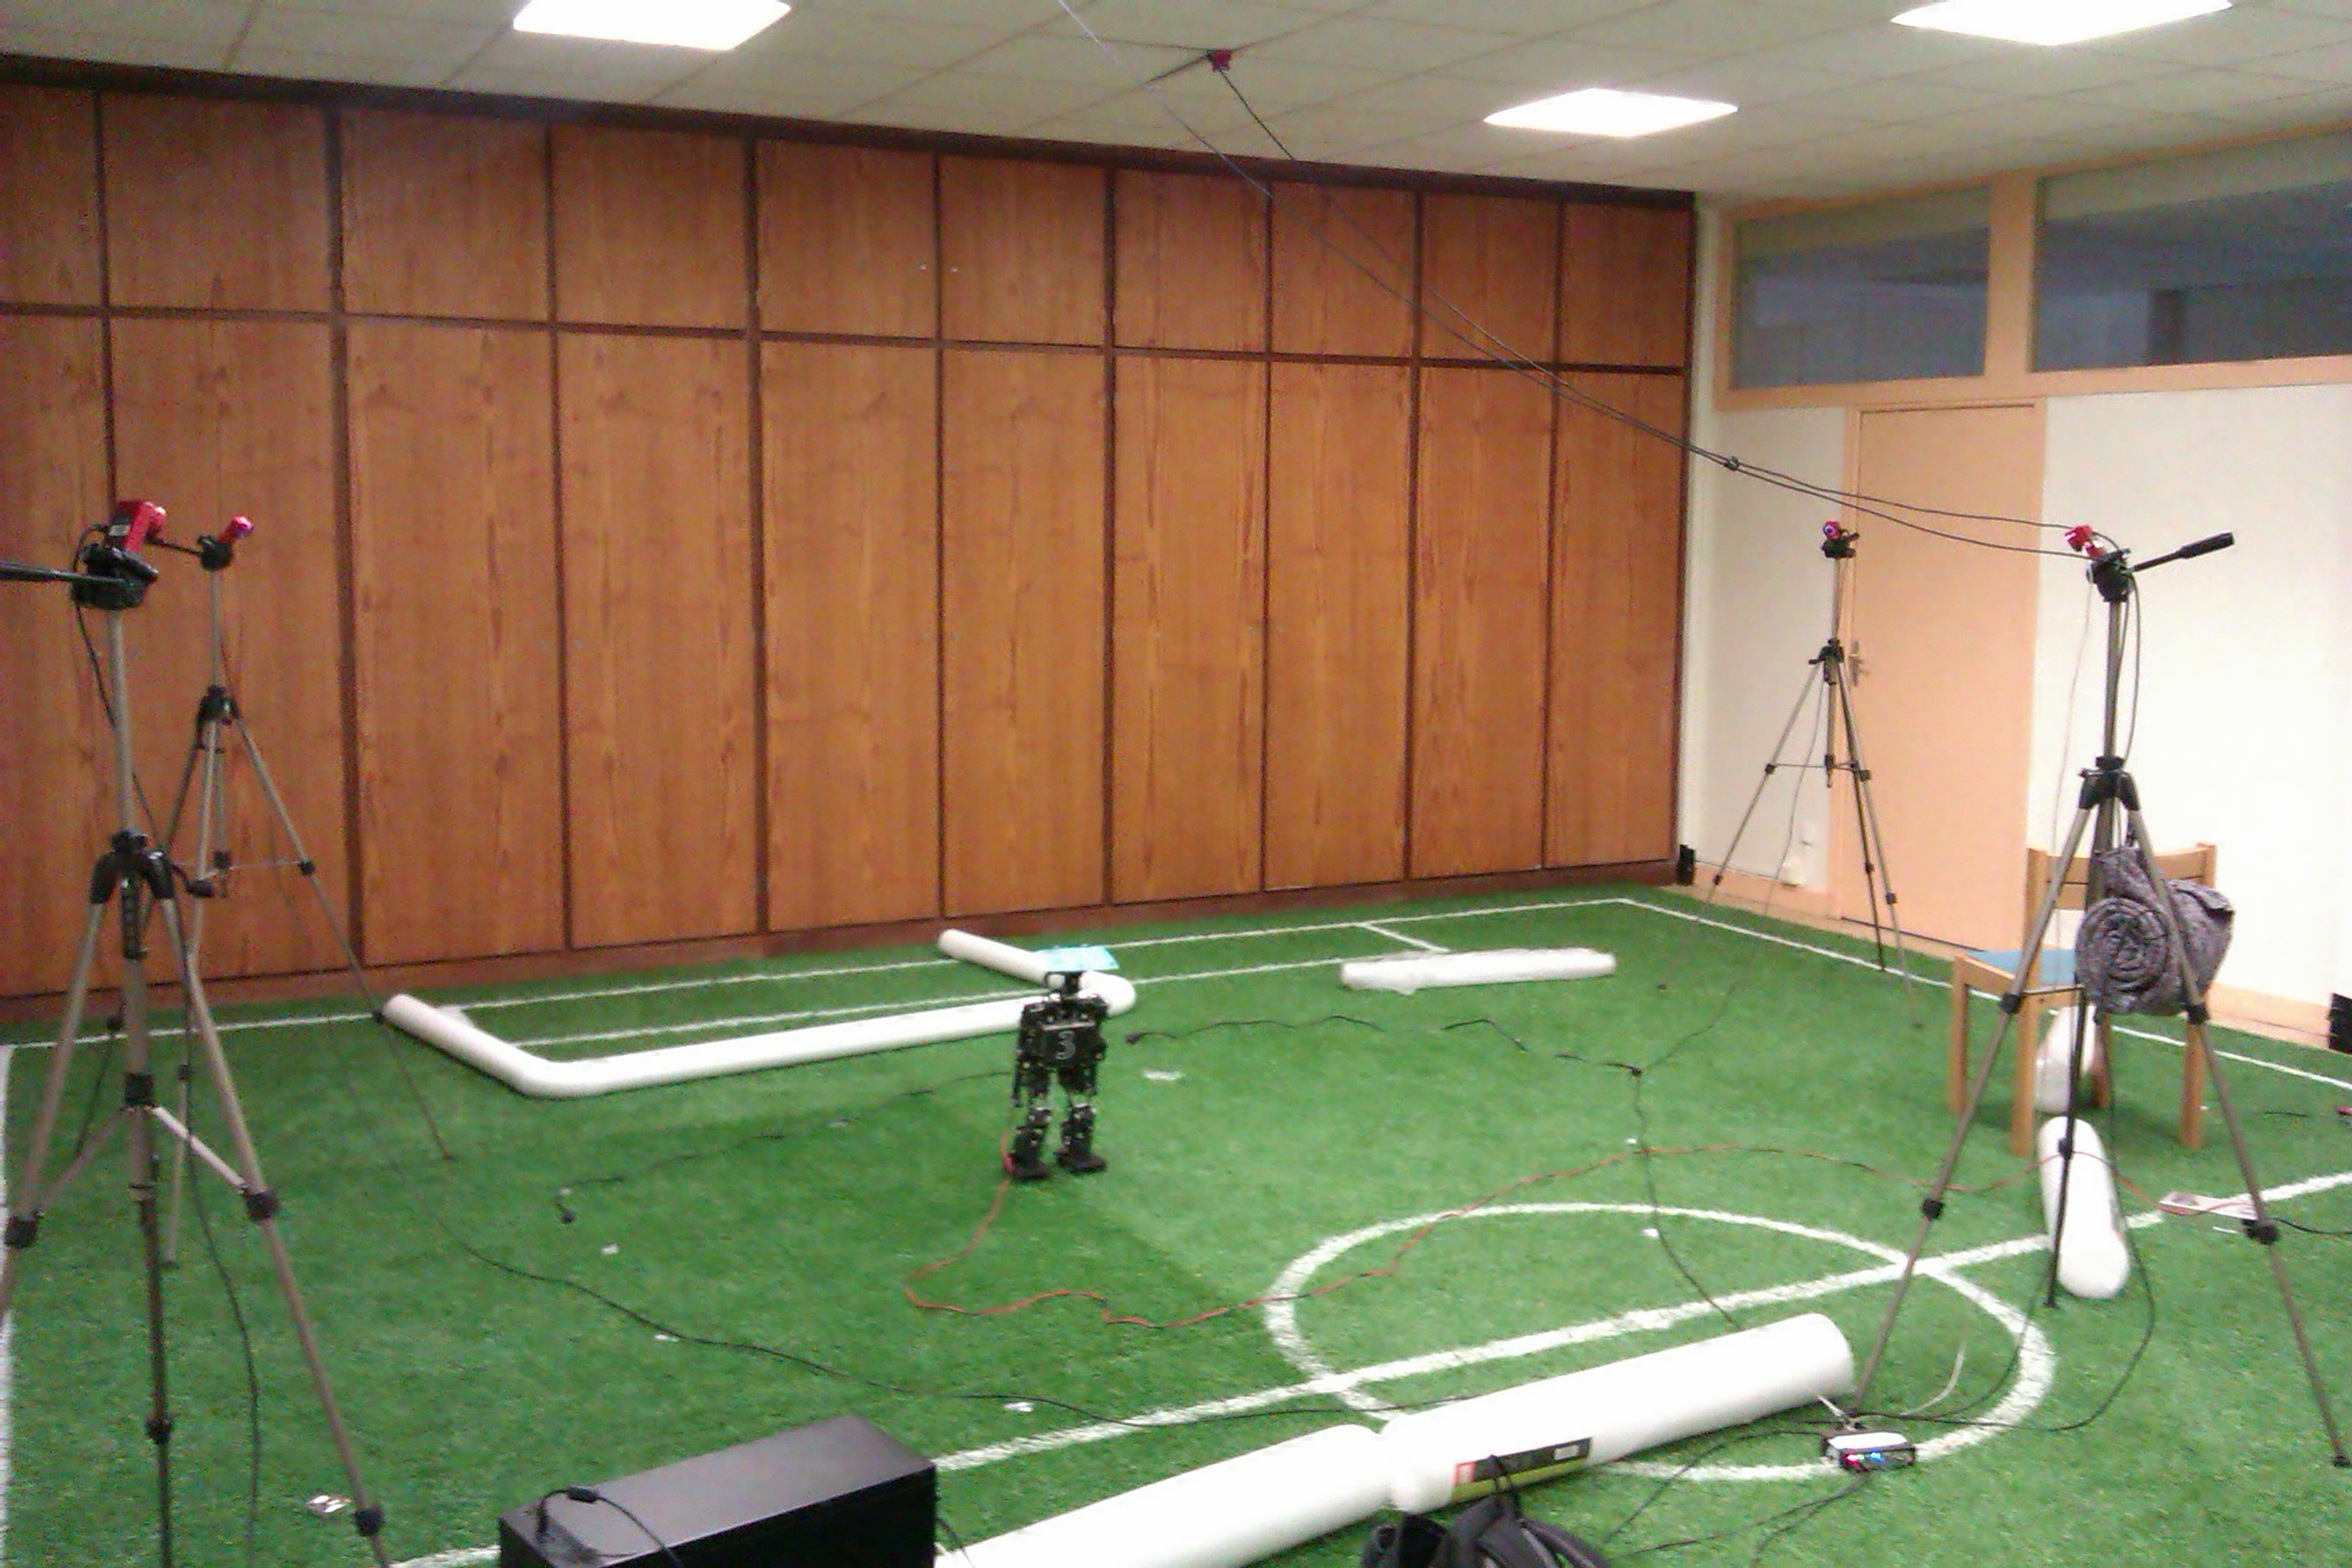
\includegraphics[width=1.0\linewidth]{../media/mocap_setup1.jpg}
        \end{column}
    \end{columns}
\end{frame}

\begin{frame}{Apprentissage des fonctions de correction}
    $\Delta \bm{p}_{t}^{\text{read}} \in \mathbb{R}^3$ : estimation déplacement égocentrique proprioceptive au pas $t$\\
    $\Delta \bm{p}_{t}^{\text{mocap}} \in \mathbb{R}^3$ : mesure déplacement égocentrique au pas $t$\\
    $s_{t}^{\text{read}} \in \{0, 1\}$ : pied de support proprioceptif au pas $t$\\
    $l_{t} \in \mathbb{R}_{+}$ : durée du pas $t$\\
    \vspace{1em}
    Odométrie proprioceptive :
    $$
    \mathbb{R}^9 \longrightarrow \mathbb{R}
    $$
    $$
    \begin{cases}
    \big(\Delta \bm{p}_{t}^{\text{read}}, \Delta \bm{p}_{t-1}^{\text{read}}, s_{t}^{\text{read}}, l_{t}, l_{t-1}\big) 
    \longmapsto \Delta x_{t}^{\text{mocap}} \\
    \big(\Delta \bm{p}_{t}^{\text{read}}, \Delta \bm{p}_{t-1}^{\text{read}}, s_{t}^{\text{read}}, l_{t}, l_{t-1}\big) 
    \longmapsto \Delta y_{t}^{\text{mocap}} \\
    \big(\Delta \bm{p}_{t}^{\text{read}}, \Delta \bm{p}_{t-1}^{\text{read}}, s_{t}^{\text{read}}, l_{t}, l_{t-1}\big) 
    \longmapsto \Delta \theta_{t}^{\text{mocap}} \\
    \end{cases}
    $$
    Odométrie prédictive :
    $$
    \mathbb{R}^7 \longrightarrow \mathbb{R}
    $$
    $$
    \begin{cases}
    \big(\Delta \bm{p}_{t}^{\text{goal}}, \Delta \bm{p}_{t-1}^{\text{goal}}, s_{t}^{\text{goal}}\big) 
    \longmapsto \Delta x_{t}^{\text{mocap}} \\
    \big(\Delta \bm{p}_{t}^{\text{goal}}, \Delta \bm{p}_{t-1}^{\text{goal}}, s_{t}^{\text{goal}}\big) 
    \longmapsto \Delta y_{t}^{\text{mocap}} \\
    \big(\Delta \bm{p}_{t}^{\text{goal}}, \Delta \bm{p}_{t-1}^{\text{goal}}, s_{t}^{\text{goal}}\big) 
    \longmapsto \Delta \theta_{t}^{\text{mocap}} \\
    \end{cases}
    $$
\end{frame}

\begin{frame}{Régression non paramétrique LWPR}
    \begin{columns}
        \begin{column}{0.7\linewidth}
            \begin{block}{Régression non paramétrique}
                \begin{itemize}
                    \item Pas de forme imposée de la solution
                    \item Nécessite plus de données
                \end{itemize}
            \end{block}
            \vspace{1.0em}
            \textit{Locally Weighted Projection Regression} (LWPR) :
            \begin{itemize}
                \item \customtextcolor{(Vijayakumar et al., 2005)}
                \item Très peu calculatoire
                \item Réduction de dimension
            \end{itemize}
        \end{column}
    \end{columns}
\end{frame}

\begin{frame}{Contextes et expérimentations}
    \begin{columns}
        \begin{column}{0.5\linewidth}
            \vspace{1.0em}
            \begin{itemize}
                \item Herbe artificielle
                \item Pilotage manuel du déplacement
                \item Exploration de l'espace de contrôle
            \end{itemize}
            \vspace{2.0em}
            \centering
            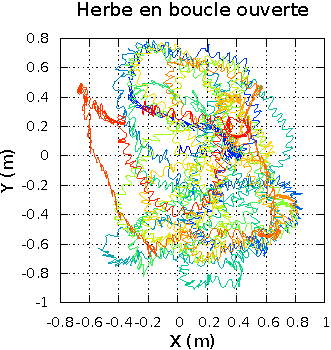
\includegraphics[type=pdf,ext=.pdf,read=.pdf,width=0.8\linewidth]{../plot/OdometryLWPR/grass_open_learn_log_complete_traj}
        \end{column}
        \begin{column}{0.5\linewidth}
            \centering
            \movie[
                autostart,
                width=\linewidth, 
                height=0.56\linewidth,
                poster,
                loop
            ]{}{../video/cutExploreICRA.mp4}
        \end{column}
    \end{columns}
\end{frame}

\begin{frame}{Résultats (1/3) -- Données et corrélations}
    \begin{columns}
        \begin{column}{0.35\linewidth}
            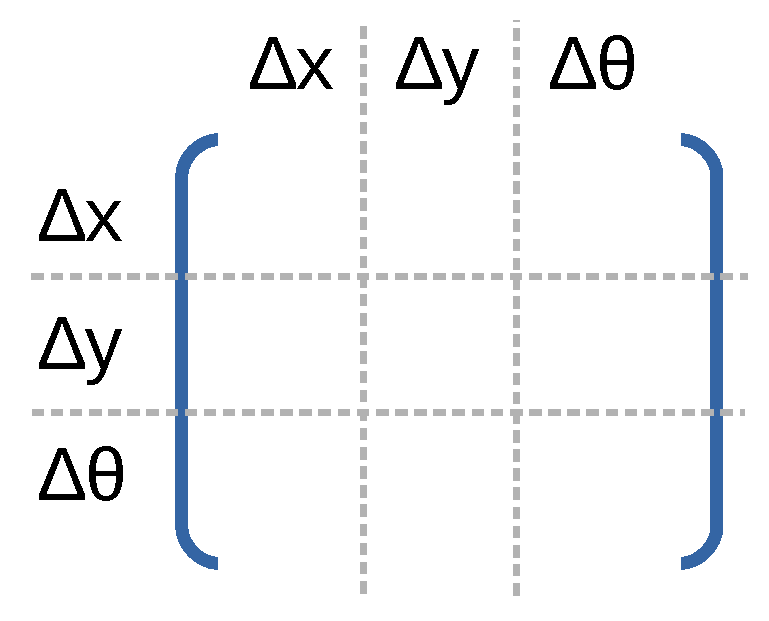
\includegraphics[type=pdf,ext=.pdf,read=.pdf,width=0.8\linewidth]{../schema/correlation_matrix}
        \end{column}
        \begin{column}{0.65\linewidth}
            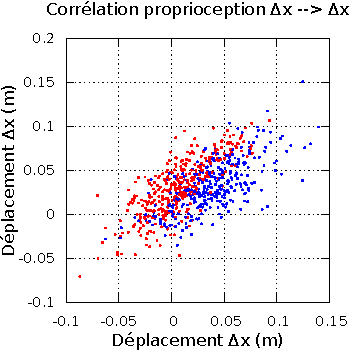
\includegraphics[type=pdf,ext=.pdf,read=.pdf,width=2.5cm]{../plot/OdometryLWPR/grass_close_function_read_x_x}
            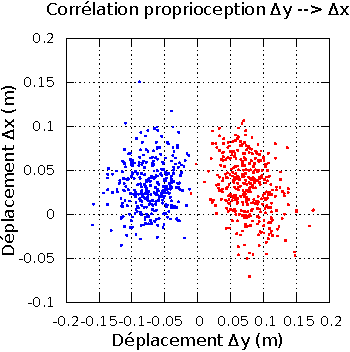
\includegraphics[type=pdf,ext=.pdf,read=.pdf,width=2.5cm]{../plot/OdometryLWPR/grass_close_function_read_y_x}
            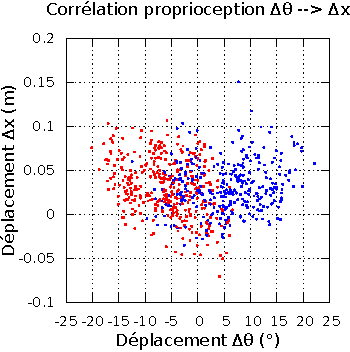
\includegraphics[type=pdf,ext=.pdf,read=.pdf,width=2.5cm]{../plot/OdometryLWPR/grass_close_function_read_yaw_x}
            \vspace{0.2cm}
            \newline
            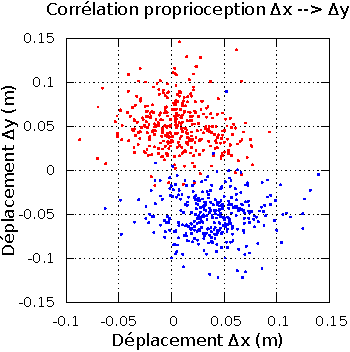
\includegraphics[type=pdf,ext=.pdf,read=.pdf,width=2.5cm]{../plot/OdometryLWPR/grass_close_function_read_x_y}
            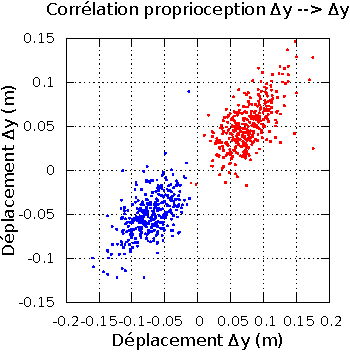
\includegraphics[type=pdf,ext=.pdf,read=.pdf,width=2.5cm]{../plot/OdometryLWPR/grass_close_function_read_y_y}
            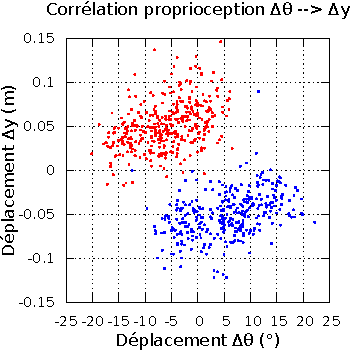
\includegraphics[type=pdf,ext=.pdf,read=.pdf,width=2.5cm]{../plot/OdometryLWPR/grass_close_function_read_yaw_y}
            \vspace{0.2cm}
            \newline
            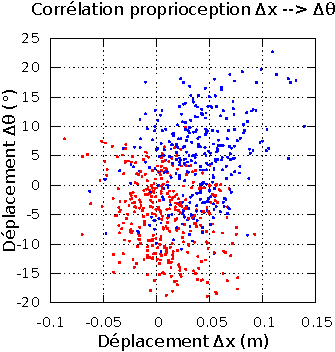
\includegraphics[type=pdf,ext=.pdf,read=.pdf,width=2.5cm]{../plot/OdometryLWPR/grass_close_function_read_x_yaw}
            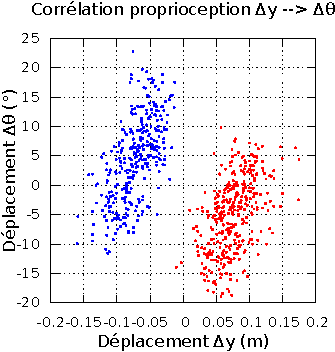
\includegraphics[type=pdf,ext=.pdf,read=.pdf,width=2.5cm]{../plot/OdometryLWPR/grass_close_function_read_y_yaw}
            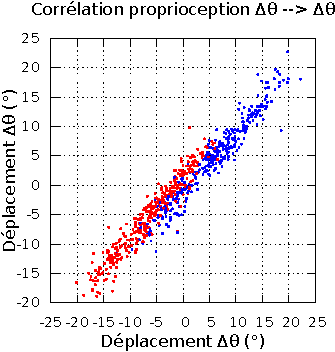
\includegraphics[type=pdf,ext=.pdf,read=.pdf,width=2.5cm]{../plot/OdometryLWPR/grass_close_function_read_yaw_yaw}
        \end{column}
    \end{columns}
\end{frame}

\begin{frame}{Résultats (2/3) -- Trajectoires estimées et statistiques}
    \begin{columns}
        \begin{column}{0.5\linewidth}
            \centering
            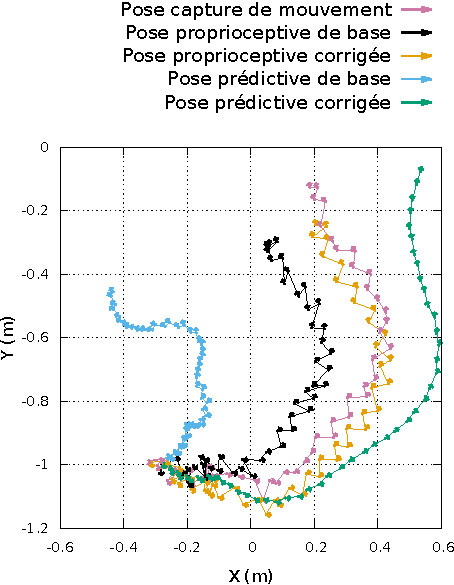
\includegraphics[type=pdf,ext=.pdf,read=.pdf,width=1.0\linewidth]{../plot/OdometryLWPR/grass_open_traj2_pose}
        \end{column}
        \begin{column}{0.5\linewidth}
            \centering
            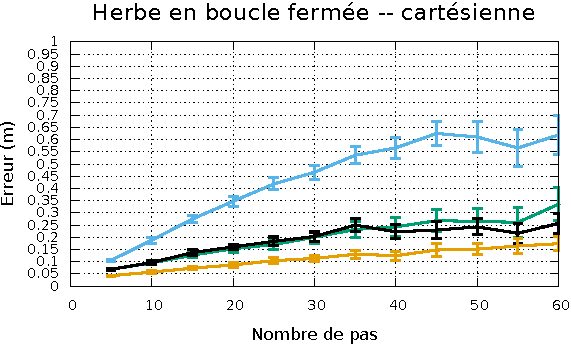
\includegraphics[type=pdf,ext=.pdf,read=.pdf,width=1.0\linewidth]{../plot/OdometryLWPR/grass_close_compare_cart}
            \begin{itemize}
                \item Fonctions de correction $\Rightarrow$ réduction de la dérive
                \item Temps de calcul embarqué (modèle + LWPR) : $8$~ms
            \end{itemize}
        \end{column}
    \end{columns}
\end{frame}

\begin{frame}{Conclusion}
    \begin{columns}
        \begin{column}{0.4\linewidth}
            Comparaison odométrie (40 pas) :
            \begin{itemize}
                \item Proprioceptive corrigée : $0.34$~m $\Rightarrow$ $\bm{0.12}$~m
                \item Visuelle \customtextcolor{(Oriolo at al., 2016)} $\Rightarrow$ $\bm{0.03}$~m
            \end{itemize}
            \vspace{1.0em}
            Cas d'utilisation :
            \begin{itemize}
                \item Temps de calcul
                \item Environnement visuel non adapté
                \item Prédiction (modèle de déplacement) :\\
                    $0.70$~m $\Rightarrow$ $\bm{0.16}$~m
            \end{itemize}
        \end{column}
        \begin{column}{0.6\linewidth}
            \centering
            \movie[
                autostart,
                width=\linewidth, 
                height=0.56\linewidth,
                poster,
                loop
            ]{}{../video/cutICRA_light.mp4}
            \scriptsize
            \definecolor{customCyan}{RGB}{6,206,200}
            \definecolor{customPurple}{RGB}{187,11,231}
            \definecolor{customBlue}{RGB}{9,124,228}
            \definecolor{customGreen}{RGB}{10,188,17}
            \definecolor{customRed}{RGB}{237,12,13}
            \newline
            \vspace{1.0em}
            \begin{tabular}{ll}
                \tikz \fill [customRed]    (0,0) rectangle (0.4,0.2); Mesure & \\
                \tikz \fill [customBlue]   (0,0) rectangle (0.4,0.2); Proprioception base &
                \tikz \fill [customGreen]  (0,0) rectangle (0.4,0.2); Proprioception corrigée\\
                \tikz \fill [customCyan]   (0,0) rectangle (0.4,0.2); Prédiction base &
                \tikz \fill [customPurple] (0,0) rectangle (0.4,0.2); Prédiction corrigée\\
            \end{tabular}
        \end{column}
    \end{columns}
    \begin{block}{}
        \customtextcolor{
            \small
            \textit{Learning the odometry on a small humanoid robot}}\\
        \scriptsize
        Quentin Rouxel, Grégoire Passault, Ludovic Hofer, Steve N'Guyen, Olivier Ly\\
        ICRA, 2016
    \end{block}
\end{frame}

